\section{Transformers}
Doğal Dil İşleme (NLP) alanında son yıllarda yaşanan en heyecan verici gelişmelerden biri Transformers adı verilen bir yapay zeka modeli ve algoritma ailesinin ortaya çıkmasıdır. Transformers, derin öğrenme alanında büyük bir çığır açarak NLP uygulamalarında büyük bir devrim yaratmıştır.

\begin{figure}[ht]
    \centering
    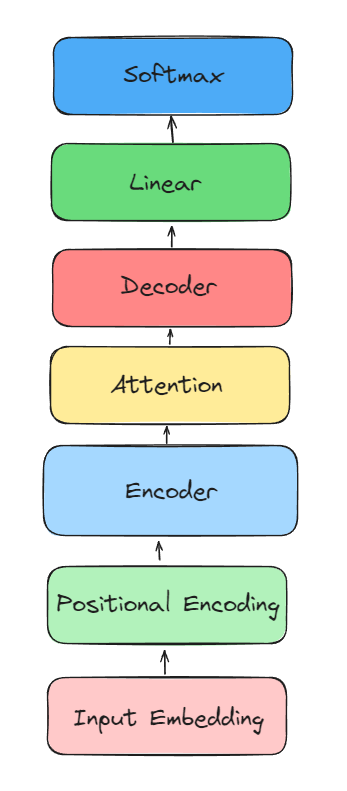
\includegraphics[width=0.5\textwidth]{images/transformer_architecture.png}
    \caption{Transformers mimarisi.}
    \label{fig:enter-label}
\end{figure}

Transformers, derin öğrenme modellerinde kullanılan bir sinir ağı mimarisidir. 2017 yılında Google tarafından geliştirilen ve “Attention is All You Need” başlıklı makalede tanıtılan dönüşümler, özellikle dil modelleri ve çeviri sistemleri gibi doğal dil işleme görevlerinde büyük başarı elde etmiştir. Geleneksel dil işleme modellerinden farklı olarak, Transformers birçok dil işleme görevinde tek bir model kullanarak state-of-the-art sonuçlar elde etmiştir. Seq2Seq modellerinde karşılaşılan bağlam kaybı problemlerine etkili bir çözüm sunar. Bu problemi aşmak için Attention (Dikkat) Mekanizmasını kullanır.

Bir Transformers ağında aşağıdaki bileşenler bulunur:
\begin{itemize}
    \item \textbf{Encoder-Decoder Yapısı:} Encoder, girdi verisini içsel temsillere dönüştürür. Decoder, bu içsel temsilleri çıktıya dönüştürür.
    \item \textbf{Attention Mekanizması:} Modelin belirli bir kelimenin işlenmesi sırasında diğer kelimelere odaklanmasını sağlar. Bu sayede, modelin girdi verisindeki uzak bağlantıları da dikkate alması mümkün olur.
    \item \textbf{Layer Normalization ve Residual Connections}
    \item \textbf{Positional Encoding:} Girdi verisindeki kelime sıralamasını koruyabilmek için bir pozisyon kodlaması kullanır.
\end{itemize}

\subsection{Attention Mekanizması}
Attention mekanizması, kod çözücü ağının her adımında, her bir giriş kelimesine odaklanmasına izin vererek çalışır. Yani kod çözücü ağı çıkışın her bir kelimesini oluştururken, giriş dizisindeki her bir kelimenin önemini değerlendirir ve çıkışın o kelimeyi üretirken girişin hangi kısımlarına odaklanması gerektiğin karar verir.

\subsection{Encoder}
Encoder, girdi verisini içsel temsillere dönüştürür. Bunu gerçekleştirmek için encoder bloğu, word embedding, positional encoding, multi-head attention, normalizasyon ve bir dizi lineer katman kullanır.

\subsection{Word Embedding}
Kelimelerin anlamsal benzerliklerini yansıtacak şekilde gömümlere dönüştürülmesidir. Bu sayede kelimeler anlamsal benzerliklerini koruyarak modelin işleyebileceği sayısal verilere dönüştürülür.

\subsection{Positional Encoding}
Positional encoding, kelimelerin sıra bilgisini koruyarak sayısal vektörlere dönüştürülmesidir. Bu sayede model kelimeler arası ilişkileri daha iyi anlayabilir. Word embedding işleminden çıkan gömümler ile positional encoding işleminden çıkan vektörler toplanır. Böylece, girdi içerisinde hem anlam bilgisi hem sıra bilgisi barındırılır.

\[\text{PositionalEncoding}(pos, i) = \begin{cases}
    \sin\left(\frac{pos}{10000^{2i/d_{\text{model}}}}\right) & \text{if } i \text{ is even} \\
    \cos\left(\frac{pos}{10000^{2i/d_{\text{model}}}}\right) & \text{if } i \text{ is odd}
\end{cases}\]

\subsection{Multi-Head Attention}
Positional encoding katmanından gelen girdi verisi key, value ve query olmak üzere üç farklı kanaldan iletilir ve daha sonra her bir kanalda lineer katmanlardan geçer. 
\begin{itemize}
    \item \textbf{Key:} Key kanalı, dikkat odaklamasının hangi kelimelerin dikkate alınacağını belirlemek için kullanılır. Her bir kelimenin içsel temsili, key kanalı tarafından temsil edilir ve dikkat ağırlıklarının hesaplanmasında kullanılır
    \item \textbf{Query:} Query kanalı, dikkat odaklamasının hangi kelimelere odaklanacağını belirlemek için kullanılır. Her bir kelimenin içsel temsili, query kanalı tarafından temsil edilir ve dikkat ağırlıklarının hesaplanmasında kullanılır.
    \item \textbf{Value:} Value kanalı, dikkat ağırlıklarının hesaplanmasından sonra kullanılarak dikkat odaklamasının sonucu olarak elde edilen temsilin oluşturulmasında kullanılır. Dikkat ağırlıkları ile ağırlıklı olarak çarpılan her bir kelimenin içsel temsili, value kanalı tarafından temsil edilir.
\end{itemize}
Multi-head attention denmesinin sebebi, positional encoding katmanından gelen veriler birden fazla bloktan geçer ve çıktıları birleştirilir. Son temsili elde etmek için doğrusal olarak dönüştürülür.

\subsection{Residual Connections}
Residual connections, modelin daha derin hale getirilmesini sağlar ve aşırı öğrenmeyi önler. Bu bağlantılar, bir katmanın girdi verisini alır ve o katmandan çıkan çıktıyı girdi verisi ile toplar. Bu sayede, katmanların doğrudan öğrenmesi gereken bir araç vardır ve gradientlerin daha iyi akması sağlanır.

\subsection{Layer Normalization}
Layer normalization, her bir katmanın çıktılarını normalize ederek modelin daha kararlı ve tutarlı bir şekilde eğitilmesini sağlar. Bu, her bir katmanın çıktılarının ortalamasını sıfıra merkezlemek ve birim varyans ile ölçeklemek suretiyle gerçekleştirilir.

\subsection{Decoder}
İlk olarak, başlangıç tokeni decoder'a girdi olarak verilir. Bu başlangıç tokeni, decoder'a çevirilecek cümlenin başlangıcını belirtir. Başlangıç tokeni, self-attention mekanizması kullanılarak işlenir. Bu adımda, başlangıç tokeninin içsel temsili hesaplanır ve diğer kelimelere dikkat edilerek daha karmaşık bir temsil elde edilir. Self-attention adımından sonra, decoder bloğu, encoder bloğundan gelen çıktıları dikkate alır. Bu adımda, encoder-decoder attention mekanizması kullanılarak encoder bloğunun çıktılarına dikkat edilir. Her bir attention adımından sonra, decoder bloğunda layer normalization ve residual bağlantılar kullanılır. Bu teknikler, modelin daha kararlı bir şekilde eğitilmesine ve aşırı öğrenmeyi önlemesine yardımcı olur. Son olarak, her bir attention adımından sonra, decoder bloğunda bir ileri beslemeli sinir ağı (feed-forward neural network) bulunur. Bu ağ, içsel temsilleri daha karmaşık ve yüksek seviyeli bir şekilde işlemek için kullanılır. İleri beslemeli sinir ağı adımından sonra, sonlandırma tokeni decoder'a girdi olarak verilir. Bu sonlandırma tokeni, decoder'ın çıktı oluşturma işlemini sonlandırır ve decoder'ın çıktı dizisini tamamlar.

\newpage